% Load Latin Modern before the class: quantumarticle only pulls it in
% \AtBeginDocument, which is too late for ltxgrid's saved column font state
% on this TeX Live (body would silently fall back to bitmap EC fonts).
\RequirePackage{lmodern}
\documentclass[a4paper,twocolumn,11pt,unpublished]{quantumarticle}
\pdfoutput=1

\usepackage[utf8]{inputenc}
\usepackage[T1]{fontenc}
\usepackage{amsmath,amssymb,amsthm}
\usepackage{booktabs}
\usepackage{graphicx}
\usepackage[numbers,sort&compress]{natbib}
\usepackage{hyperref}

% Local shim: without a full revtex install the vendored ltxgrid/ltxutil copies
% interact badly with the modern LaTeX kernel's end-document hooks. Harmless on
% a proper install (texlive-publishers); see compile.sh.
\makeatletter
\providecommand{\@afterenddocumenthook}{}
\makeatother

\theoremstyle{plain}
\newtheorem{proposition}{Proposition}
\newtheorem{lemma}[proposition]{Lemma}
\newtheorem{corollary}[proposition]{Corollary}
\theoremstyle{remark}
\newtheorem{remark}[proposition]{Remark}

\newcommand{\geo}{\mathrm{geo}}
\newcommand{\vecop}{\operatorname{vec}}
\newcommand{\rk}{\operatorname{rank}}
\newcommand{\ket}[1]{|#1\rangle}
\newcommand{\braket}[2]{\langle#1|#2\rangle}
\newcommand{\amp}[3]{\langle#1|\,#2\,|#3\rangle}
\newcommand{\Zspec}{Z_{\mathrm{spec}}}
\newcommand{\ZDW}{Z_{\mathrm{DW}}}
\newcommand{\kerL}{\ker L}

\title{Realizing quantum gates as triangulated cobordisms: a
conservation-law gate set and machine-precision transition amplitudes}

\author{Andrew Kelleher}
\affiliation{Independent researcher}  % TODO: confirm affiliation / add \orcid{}
\email{keats.kelleher@gmail.com}

\begin{document}

\maketitle

\begin{abstract}
Which quantum gates can be realized as discrete geometries --- triangulated
cobordisms whose boundary carries the states and whose field-theoretic value
is the transition amplitude --- and how accurately do those geometries
reproduce the amplitudes? We give a variational answer: the gate is bent to
a boundary state by the Choi--Jamio{\l}kowski isomorphism, the boundary
geometry is held fixed, and the bulk interior (edge weights and, through
growth and surgery moves, topology) is synthesized by driving a
Hodge-Laplacian eigenvector residual to zero; non-realizability is certified
by a residual floor rather than by exhausting triangulations. On a
$\mathbb{Z}_2$ holonomy register carried by a triangulated sphere opened by
surgery, we prove the realizable gate actions are exactly those whose
holonomy block conserves total charge --- a continuous group, with $S_3$,
$H\otimes H$, the controlled-$\sqrt{X}$ family, and the
$\sqrt{\mathrm{SWAP}}$ roots among its named members --- and prove that a
cyclic symmetry of the holes forces the carried chart to be an isometry,
so the anchored Hodge pairing \emph{is} the operator transition
amplitude. The synthesized registers realize these hypotheses at machine
precision: the criterion decides all $52$ battery gates and all $1443$
genuine registers in $3300$ randomized bulk draws, the value matches the
amplitude to $5.0\times10^{-16}$, survives a symmetry-preserving
re-triangulation exactly, and deviates on anisotropic bulks by precisely
the proven Gram-defect law. Obstructed gates admit no value at all.
\end{abstract}

\section{Introduction}
\label{sec:intro}

Given a quantum operation $U:\mathcal{H}_B\to\mathcal{H}_A$ between two
states, does a discrete geometry exist that \emph{is} that operation --- a
triangulated cobordism $W_{AB}$ whose boundary is the two state geometries
and whose value at the pair is the transition amplitude --- and can such a
geometry be found, or its non-existence certified, by an algorithm? The
question is the computational converse of functorial field theory, which
assigns state spaces to boundaries and linear maps to the manifolds
interpolating between them \cite{Atiyah1988TQFT,Segal2004Definition}:
states prepared by bounding geometries
\cite{HartleHawking1983WaveFunction}, amplitudes assigned to general
boundaries \cite{Oeckl2003GeneralBoundary}.

This paper develops and validates a variational answer. The correspondence
under test consists of three hypotheses:
\begin{align}
  \textbf{H1:}\quad & W_{AB}=\geo(U) \text{ is a cobordism},\\
  \textbf{H2:}\quad & \partial W_{AB}
      = \overline{\geo(\psi_B)}\sqcup\geo(\psi_A),\\
  \textbf{H3:}\quad & Z(W_{AB})=\amp{\psi_A}{U}{\psi_B},
  \label{eq:h3}
\end{align}
with the rank refinement that $\rk(U)$ equals the operator-Schmidt rank
of $\vecop(U)$ \cite{Nielsen2003DynamicsResource}, which equals the
connectivity of $W_{AB}$. Since transition probabilities are
$p=|\amp{\psi_A}{U}{\psi_B}|^2$ for normalized states, a method that
reproduces amplitudes at machine precision reproduces the probabilities at
the same order.

\emph{What $\geo$ denotes.} $\geo(\psi)$ is a \emph{carrier} of the state
$\psi$: a Hermitian-weighted simplicial complex whose Laplacian has
$\psi$ as a distinguished eigenvector (made precise in
Sec.~\ref{sec:method}); $\geo(U)$ is a carrier of the bent state
$\vecop(U)$, synthesized with its boundary pinned; the overline in H2 is
orientation reversal. $\geo$ is our notation, not a previously defined
map, and it is not canonical: carriers need not exist --- H1 \emph{is}
the existence question, and the obstructions of
Sec.~\ref{sec:results-h1} are its failures --- and are never unique
(every genuine register of Sec.~\ref{sec:results-gates} carries the same
gates). $\geo(\cdot)$ denotes the witness the synthesis returns. What
\emph{is} canonical runs the other way --- the field-theoretic
assignment of a boundary state to a bounding geometry
\cite{Atiyah1988TQFT,HartleHawking1983WaveFunction,Oeckl2003GeneralBoundary}
--- and a carrier is a pointwise section of it, found variationally;
choosing \emph{among} carriers is deliberately deferred to the
mediated-synthesis program of the Outlook.

Our contributions are:
\begin{enumerate}
\item \textbf{A residual method for finding the cobordism.} The operation
  is bent to a boundary state by the Choi--Jamio{\l}kowski isomorphism
  \cite{Choi1975CompletelyPositive,Jamiolkowski1972LinearTransformations,AbramskyCoecke2004Categorical};
  the boundary is pinned bitwise-identically; and the interior ---
  Hermitian edge weights together with topology-changing moves
  (boundary-fixed cone growth, interior-cell surgery, and their
  composition) --- is optimized to drive the eigenvector residual
  $r(W)=\lVert(I-\psi\psi^\dagger)L\psi\rVert^2$ to zero
  (Sec.~\ref{sec:method}).
\item \textbf{Certified obstructions.} Non-realizability is established by
  a residual \emph{floor}: seed-independent and, for the principal witness,
  equal to $2/85$ to machine precision and cross-checked against an
  independent global minimization over its single interior parameter
  (Sec.~\ref{sec:results-h1}). These are numerical certificates ---
  seed-independence plus independent minimization --- not analytic proofs
  of obstruction; the gap to provable obstructions is discussed in the
  Outlook. Existence is decided by certificates, not by enumeration of
  triangulations.
\item \textbf{A proven conservation-law gate set.} On a $\mathbb{Z}_2$
  holonomy register carried by a surgery-opened triangulated sphere, a
  gate's register action is realizable precisely when its holonomy-class
  block conserves total charge. We prove this
  (Proposition~\ref{prop:register} and Lemma~\ref{lem:criterion}): the
  surgered topology forces the carried subspace to be the charge-zero
  period hyperplane, and preserving a hyperplane is a column-sum
  condition --- a continuous group, not a finite list. The implementation
  confirms the theorem on all $1443$ genuine registers found among
  $3300$ randomized bulk draws, including additive refinements; the
  remaining draws fall outside the proposition's hypothesis and saturate
  the period space, dissolving the register rather than carrying a new
  gate (Sec.~\ref{sec:results-gates}).
\item \textbf{Transition amplitudes as an exact identity.} The value of
  the cobordism is the Hodge inner product of carried harmonic
  representatives with one global scale fixed by the identity (cylinder)
  anchor. We prove that a cyclic simplicial symmetry of the holes ---
  which the canonical register possesses, verifiably --- forces the
  carried chart to be an isometry, so the anchored pairing equals the
  operator amplitude identically, and that on an anisotropic chart the
  deviation obeys an exact Gram-defect law
  (Propositions~\ref{prop:isometry}, Lemma~\ref{lem:value}). The
  experiments validate the pipeline end-to-end: worst-case deviation
  $5.0\times10^{-16}$ across all realized gates and state pairs, exact
  carry-over to a symmetry-preserving re-triangulation, and generic-draw
  deviations matching the proven law at the same precision
  (Sec.~\ref{sec:results-h3}).
\end{enumerate}

\emph{Assumptions and scope.} The register is abelian: $\mathbb{Z}_2$
holonomy on a torus boundary, with a two-dimensional carried subspace.
``Realized'' throughout means the gate's action on that carried register
--- its $\{[a],[b],[a{+}b]\}$ holonomy block restricted to the $\Sigma=0$
subspace --- not the full two-qubit unitary on $\mathbb{C}^4$. The
synthesized bulks are finite Hermitian-weighted simplicial complexes with
pinned boundary: graphs (1-complexes) for the H1 witnesses of
Sec.~\ref{sec:results-h1}, surfaces-with-boundary (2-complexes) for the
register experiments; PL-manifoldness is \emph{not} verified (no link
condition is checked), and randomized surgery draws need not remain
manifolds. The named count of realizable gates tracks the chosen battery;
the criterion is the result. The value reading requires an isometric
register chart: Section~\ref{sec:theorems} proves a cyclic hole symmetry
suffices and verifies it for the canonical bulk; the symmetry is
sufficient, not claimed necessary, and which asymmetric bulks also
furnish isometric charts is charted only empirically.

Throughout, the decision layer is purely spectral: eigendecompositions of
metric Hodge Laplacians on the triangulation. A finite-group state-sum
layer (Dijkgraaf--Witten theory \cite{DijkgraafWitten1990Topological}) was
used historically to calibrate the construction and reappears here only as
a cross-check; the data show its invariant to be the integer-quantized
shadow of the continuous spectral value (Sec.~\ref{sec:dw}).

\section{Relation to prior work}
\label{sec:related}

The correspondence itself is the Atiyah--Segal reading of field theory
\cite{Atiyah1988TQFT,Segal2004Definition} on discrete data; what is
tested here is whether a concrete simplicial machine realizes it, and
whether realizability can be \emph{decided}. Three strands of prior work
bound the contribution.

\emph{Which gates does a topological theory realize?} This is the founding
question of topological quantum computation
\cite{Freedman2003TQC,FreedmanKitaevWang2002Simulation,FreedmanLarsenWang2002Universal}.
For abelian theories the braiding/mapping-class image is finite
(property~F \cite{NaiduRowell2011PropertyF}); consistently, the pinned
(fixed-topology) image in the Dijkgraaf--Witten calibration layer of this
construction is exactly the six holonomy permutations $S_3$
(Sec.~\ref{sec:dw}). The enlargement we obtain by synthesizing the boundary
--- topology change as the computational move --- has established cousins
in lattice surgery \cite{Horsman2012LatticeSurgery} and in twist defects
and genons in abelian phases
\cite{Bombin2010Twist,BarkeshliJianQi2013TwistDefects}, formulated there
in stabilizer-code language; here the same theme appears in spectral
language, and what survives topology change is governed by a conservation
law rather than a code deformation. The question itself --- which
entangling gates arise as representations of a topological or algebraic
structure --- has direct precedent in this journal
\cite{Padmanabhan2020Braiding}, as does the identification of quantum
processes with discrete path integrals on spacetime lattices
\cite{Bauer2024FixedPoint}.

\emph{Laplacian data in topological field theory.} Classically, Laplacians
enter as determinant prefactors: abelian BF/Chern--Simons partition
functions equal Ray--Singer analytic torsion
\cite{RaySinger1971RTorsion,Schwarz1978Torsion,Witten1989Jones},
reproduced exactly on triangulations by simplicial Hodge theory
\cite{Adams1996RTorsion,Adams1997DoubledCS}. Harmonic zero modes serve
as the abelian Chern--Simons state space in canonical quantization
\cite{BosNair1989Blocks}; cellular BF theory constructs boundary state
spaces from the cohomology of a cellular cobordism
\cite{CattaneoMnevReshetikhin2020Cellular}; and projection onto
$\kerL_k$ with overlaps against harmonic representatives is the
operational core of quantum topological-data analysis
\cite{Lloyd2016TopologicalData,Hayakawa2022Persistent,Gyurik2022TDA},
where the projection success is itself a transition probability. Even
deciding whether $\kerL_k$ is nontrivial (homology detection) is
QMA$_1$-hard for implicitly specified clique complexes
\cite{CrichignoKohler2024Clique}; the complexes here are explicit and
small, so each verdict is exact linear algebra --- the hardness result
frames the general decision problem and forecloses any efficiency claim,
motivating certificates over enumeration, nothing more. Relative to this
neighborhood, the step taken here is to read the \emph{amplitude itself}
as an anchored Hodge pairing of carried harmonic representatives on a
synthesized cobordism, to prove when that reading must equal the operator
amplitude (Sec.~\ref{sec:theorems}), and to validate it there at machine
precision.

\emph{Realizability with certificates.} Deciding which boundary
\emph{operators} admit an interior geometry, with non-existence certified
by obstructions, is completely solved for circular planar resistor
networks \cite{CurtisIngermanMorrow1998Circular}; existence-as-
optimization with rigorous certificates organizes the quantum marginal
problem \cite{Yu2021MarginalHierarchy}; which boundary data admit a bulk
geometry is the holographic entropy cone \cite{Bao2015EntropyCone}; and
least-squares formulations of inverse spectral problems are canonical
\cite{ChuGolub2005InverseEigenvalue}. The instantiation here --- an
eigenvector-residual floor over synthesized simplicial bulks,
cross-checked against an independent global minimum --- combines these
ingredients in a setting where the realized object is a quantum operation
and the certified quantity is a transition amplitude.

\section{The construction}
\label{sec:method}

\emph{Terminology.} ``Triangulated cobordism'' in this paper denotes a
finite Hermitian-weighted simplicial complex with a distinguished,
bitwise-pinned boundary pair; we verify boundary preservation (H2) and the
value equation (H3) on these objects, but PL-manifoldness is not verified.
``Bitwise-identical'' boundary pinning means every boundary cell's weight
and phase data are unchanged, byte for byte, through every interior move;
the term is used in this fixed sense throughout.

\subsection{States, operations, and bending}

A \emph{carrier} of a state $\psi$ on $d$ levels is a Hermitian-weighted
simplicial complex whose weighted graph Laplacian (at $k=0$) or metric
Hodge Laplacian $L_k$ (at $k\ge1$) has $\psi$ as a distinguished
eigenvector --- for the register layer below, a \emph{harmonic},
$\psi\in\kerL_k$, in the sense of discrete Hodge theory
\cite{Eckmann1945Harmonische,Lim2020HodgeLaplacians}; $\geo(\psi)$
denotes the carrier returned by the synthesis of
Sec.~\ref{sec:boundary}. An operation
$U:\mathcal{H}_B\to\mathcal{H}_A$ is bent to the boundary state
$\vecop(U)$ (row-major; normalized) by the Choi--Jamio{\l}kowski
isomorphism --- categorically, $\vecop(U)$ is the \emph{name} of the
morphism $U$ \cite{AbramskyCoecke2004Categorical}; the carrier of a
state has no standard counterpart --- and $\geo(U)$ is a carrier of
$\vecop(U)$. The operator-Schmidt rank of $\vecop(U)$
\cite{Nielsen2003DynamicsResource} then matches the connectivity demanded
of the bulk: rank-one operations factor through the unit object and bend
to separable states carried by disconnected cobordisms.

\subsection{Boundary synthesis}
\label{sec:boundary}

Boundary geometries are found by an inverse eigenvector problem: grow the
\emph{simplest} complex whose Laplacian carries the target state. A
general-amplitude qubit $\psi=(\sqrt{0.8},\sqrt{0.2})$ is not an
eigenvector of any two-vertex complex --- the seed floors at
$r=3.60\times10^{-3}$, with the analytic floor
$w_{\min}^2(|c_0|^2-|c_1|^2)^2$ --- and is synthesized on the minimal
triangle $K_3$ at $r=9.39\times10^{-10}$, eigenvalue $\lambda=0.199908$.
The minimal vertex count is recorded as the state's combinatorial
complexity.

\subsection{The residual oracle}
\label{sec:oracle}

Given the bent target and an assembled bulk whose boundary is pinned
bitwise-identically, the oracle minimizes the eigenvalue-agnostic residual
\begin{equation}
  r(W)\;=\;\bigl\lVert (I-\psi\psi^\dagger)\,L\,\psi \bigr\rVert^2,
  \label{eq:residual}
\end{equation}
over (i) interior Hermitian edge weights (magnitudes in $[0.1,10]$, U(1)
phases at $k=0$) and free auxiliary amplitudes, by bounded multi-restart
Levenberg--Marquardt; and (ii) interior topology, through three
boundary-fixed growth modes: \emph{cone growth} --- a stellar (Pachner
$1\to3$) subdivision adding an interior vertex
\cite{Pachner1987Bistellar,Pachner1991Shellings}; \emph{surgery} ---
removal of an interior top cell, which is \emph{not} a Pachner move (it
changes the topology by design, with $\partial W$ held
bitwise-identical); and their composition, in which each growth step
commits the best strictly-improving cut and falls back to an added vertex
otherwise, with the additive budget capped (default $20$ added vertices).
For the register layer the criterion is sharpened to the harmonic residual
$\lVert L_k\psi\rVert^2$ --- distance from $\kerL_k$ --- so that
``realizable'' means \emph{carried by the homology of the bulk}. A target
is realizable iff the residual is driven below $\epsilon=10^{-10}$
($10^{-9}$ on the register layer); an obstruction is a floor bounded above
$10^{-2}$.

Every result below verifies $\partial W$ bitwise-identical before and
after synthesis --- the boundary-preservation half of H2; the
orientation-reversed disjoint-union reading
$\partial W_{AB}=\overline{\geo(\psi_B)}\sqcup\geo(\psi_A)$ holds by
construction of the pinning rather than as a separate test.

\subsection{The register and the staged synthesis}
\label{sec:register}

The gate experiments use the torus holonomy register
$\mathbb{C}^4=\mathbb{C}[H^1(T^2;\mathbb{Z}_2)]$, whose three nontrivial
classes $\{[a],[b],[a{+}b]\}$ are carried as vertex-disjoint boundary
1-cycles on a triangulated sphere (the icosahedron in the canonical
register). The staged synthesis proceeds per gate $U$: (1) synthesize
$\geo(\psi_A)$ and $\geo(\psi_B)$ independently; (2) pin their union as
$\partial W$; (3) grow the bulk by surgery --- opening the three holonomy
holes raises $b_1$ from $0$ to $2$, and $\kerL_1$ \emph{emerges} as the
two-dimensional carried register $V$ --- and decide by the exact
eigendecomposition of $L_1$. The carried subspace is the $\Sigma=0$
hyperplane of the three holonomy-cycle periods (with induced-orientation
signs), so the post-interaction state $U\ket{\psi_B}$ is carried iff its
periods conserve total charge; this emergence and the charge constraint
are forced by the topology alone (Proposition~\ref{prop:register}). The
identity provides the falsifiable anchor: it floors
($r\approx1.1\times10^{1}$) on every seed with $\dim\kerL_1<2$ and reaches
machine zero ($r\approx10^{-29}$) only once surgery has grown the full
register.

\subsection{The value of the cobordism}
\label{sec:value}

The spectral value at a boundary pair is defined directly on the carried
harmonics. Let $h(p)$ denote the $\kerL_1(W)$ representative with
(signed) periods $p$, and let $\psi_B$ be the fixed reference input (the
$V$-generic state used throughout the battery). Then
\begin{equation}
  \Zspec\bigl(W;\psi_A,U\psi_B\bigr)
  \;=\;
  s\,\bigl\langle h(p_A),\,h(u\,p_B)\bigr\rangle,
  \label{eq:zspec}
\end{equation}
where $u$ is the gate's holonomy-class block and the single global scale
$s$ is fixed once, on the reference state, by the cylinder (T1) anchor
$\Zspec(\psi_B,\psi_B)=\braket{\psi_B}{\psi_B}$, i.e.
$s^{-1}=\langle h(p_B),h(p_B)\rangle$ --- the discrete form of ``the
trivial cobordism reproduces the inner product'' \cite{Atiyah1988TQFT}.
One scalar suffices exactly when the register chart is isometric:
Proposition~\ref{prop:isometry} proves the canonical chart is, and
Lemma~\ref{lem:value} then makes \eqref{eq:zspec} the operator amplitude
identically. On an anisotropic chart a single $s$ cannot serve all
states, and the failure obeys the exact law~\eqref{eq:deviation}
(Sec.~\ref{sec:results-h3}). The register bulk carries the unit cochain
metric, verified exactly, so the pairing is the plain Hermitian
contraction. After the anchor, every number --- every pair, every gate,
every re-grown bulk --- is a prediction. H3 \eqref{eq:h3} is then a
falsifiable equality between \eqref{eq:zspec} and the operator amplitude,
computed independently through the Choi channel; transition probabilities
follow as $|\Zspec|^2$.

\section{The register theorems}
\label{sec:theorems}

The register layer admits a complete elementary theory; this section
proves it, so that the experiments of Sec.~\ref{sec:results} validate an
implementation against theorems rather than substitute for them.
Throughout, $K$ is an oriented triangulated $2$-sphere; $f_a,f_b,f_c$ are
three pairwise vertex-disjoint faces; $W=K\setminus\{f_a,f_b,f_c\}$ is
the surgered bulk; $z_k=\partial f_k$ are the three boundary cycles with
their induced orientations; cochains carry positive-definite inner
products (the register experiments use the unit metric); and
$V=\{p\in\mathbb{C}^3:\mathbf{1}^\top p=0\}$ is the charge-zero
hyperplane. A carried state is identified with its component vector $p$
on the three nontrivial holonomy classes, in the coordinates where the
charge functional is $\mathbf{1}^\top$.

\begin{proposition}[the register is topological]
\label{prop:register}
For every triangulation $K$, every vertex-disjoint hole triple, and every
positive cochain metric: $\dim\kerL_1=2$, every harmonic $h$ is closed
and coclosed, its periods $p_k=h(z_k)$ satisfy $p_a+p_b+p_c=0$, and the
period map $\kerL_1\to V$ is a linear isomorphism.
\end{proposition}

\begin{proof}
$W$ is a triangulated three-holed sphere, so $H^1(W;\mathbb{C})\cong
\mathbb{C}^2$, and discrete Hodge theory identifies $\kerL_1\cong H^1$
with harmonics closed and coclosed
\cite{Eckmann1945Harmonische,Lim2020HodgeLaplacians}. Orient the faces
of $W$ by the orientation of $K$; the fundamental $2$-chain
$F=\sum_{f\in W_2}f$ then has $\partial F=z_a+z_b+z_c$, so for closed
$h$: $p_a+p_b+p_c=h(\partial F)=(\delta_1 h)(F)=0$. If all periods
vanish, $h$ pairs to zero with $H_1(W)$ (generated by $z_a,z_b$), so $h$
is exact, $h=\delta_0 g$; an exact coclosed cochain satisfies
$\langle h,h\rangle=\langle\delta_0 g,h\rangle=
\langle g,\delta_0^* h\rangle=0$. The period map is thus injective
between spaces of equal dimension.
\end{proof}

\begin{lemma}[conservation law]
\label{lem:criterion}
For $u\in\mathbb{C}^{3\times3}$: $uV\subseteq V$ iff
$\mathbf{1}^\top u=c\,\mathbf{1}^\top$ for some $c\in\mathbb{C}$, i.e.\
iff all column sums of $u$ are equal.
\end{lemma}

\begin{proof}
$uV\subseteq V$ says the functional $\mathbf{1}^\top u$ annihilates
$V=\ker\mathbf{1}^\top$, i.e.\ is a scalar multiple of
$\mathbf{1}^\top$.
\end{proof}

\begin{corollary}[the gate set]
\label{cor:gateset}
On any bulk as in Proposition~\ref{prop:register}, a gate's register
action is realizable --- $U\ket{\psi}$ carried for every carried $\psi$
--- iff its holonomy block conserves total charge. The realizable set is
cut out by a linear condition: a continuous family, never a finite list.
\end{corollary}

\begin{remark}
\label{rem:generic}
A single test input decides membership almost surely: if
$\mathbf{1}^\top u\not\propto\mathbf{1}^\top$, the carried inputs $p$
with $up\in V$ form a proper subspace of $V$, which a $V$-generic
reference state (the battery's, by construction) avoids.
\end{remark}

\begin{proposition}[cyclic symmetry forces an isometric chart]
\label{prop:isometry}
Let the cochain metric be real, and let $\gamma$ be an
orientation-preserving simplicial automorphism of $W$ permuting the
three holes cyclically. Then the pulled-back Hodge form
$B(p,q)=\langle h(p),h(q)\rangle$ on $V$ is a positive multiple of the
flat form: the anchor-normalized Gram matrix is exactly the identity.
\end{proposition}

\begin{proof}
$\gamma$ permutes cells and preserves the metric, so it acts unitarily
on $1$-cochains, commutes with $L_1$, and preserves $\kerL_1$; being
orientation-preserving, it maps each oriented boundary cycle to the next,
so its action on period coordinates is the plain cyclic permutation
$P_\sigma$. By uniqueness of harmonic representatives
(Proposition~\ref{prop:register}), $h(P_\sigma p)=\gamma\cdot h(p)$, so
$B$ is $P_\sigma$-invariant. On $V$, $P_\sigma$ has the two distinct
conjugate eigenvalues $\omega,\bar\omega$ ($\omega=e^{2\pi i/3}$) with
eigenvectors $x,\bar x$. Invariance gives
$B(x,\bar x)=B(P_\sigma x,P_\sigma\bar x)=\bar\omega^2 B(x,\bar x)$,
so $B(x,\bar x)=0$: $B$ is diagonal in the eigenbasis. Reality of the
metric and of $L_1$ gives $h(\bar p)=\overline{h(p)}$, hence
$B(\bar p,\bar q)=\overline{B(p,q)}$, so
$B(\bar x,\bar x)=\overline{B(x,x)}=B(x,x)$: the two diagonal entries
are equal. The flat Hermitian form is invariant under the same
$P_\sigma$ and the same conjugation, so it is diagonal in the same basis
with equal entries; therefore $B$ is a positive multiple of it, and the
anchor absorbs the multiple.
\end{proof}

\begin{remark}
\label{rem:schur}
Conceptually this is Schur's lemma --- with the full $S_3$ acting, $V$ is
the irreducible standard representation and invariant inner products on
it are proportional --- but a single $3$-fold symmetry plus the reality
of the cochain complex already suffices. The canonical register
satisfies the hypothesis verifiably: its three holes are an orbit of an
order-$3$ face-axis rotation of the icosahedron, and this $C_3$ is the
full setwise stabilizer of the triple inside the $120$-element
automorphism group (a short exhaustive check, included with the paper
sources). Geodesic subdivision is natural, so the rotation lifts to the
re-placed central-child holes of the equivariant variant tested in
Sec.~\ref{sec:results-h3}; the generic hole draws admit no such symmetry.
\end{remark}

\begin{lemma}[value identity]
\label{lem:value}
Fix a carried unit reference $\psi_B$ with coordinates $b$, anchor scale
$s^{-1}=B(b,b)$, and let $G_{kl}=s\,B(e_k,e_l)$ be the anchor-normalized
Gram matrix in a flat-orthonormal basis $\{e_k\}$ of $V$. Then for every
carried $\psi_A$ (coordinates $a$) and every block $u$ with $ub\in V$,
\begin{equation}
  \Zspec-\amp{\psi_A}{U}{\psi_B}\;=\;a^\dagger\,(G-I)\,(u\,b).
  \label{eq:deviation}
\end{equation}
In particular, if $G=I$ the anchored pairing reproduces the operator
amplitude on every carried pair, and conversely.
\end{lemma}

\begin{proof}
By definition \eqref{eq:zspec}, $\Zspec=s\,B(a,ub)=a^\dagger G\,(ub)$ in
the flat-orthonormal basis. The operator amplitude in the holonomy
embedding (both states having zero trivial-class component, $u$ the
holonomy block) is the flat contraction $a^\dagger(ub)$. Subtract. For
the converse, $a$ and $ub$ range over all of $V$ as the pair and the
realizable gate vary, forcing $G=I$.
\end{proof}

\begin{corollary}[H3 on symmetric bulks]
\label{cor:h3}
On any bulk satisfying the hypotheses of
Propositions~\ref{prop:register} and~\ref{prop:isometry},
$\Zspec=\amp{\psi_A}{U}{\psi_B}$ identically, for every realizable gate
and every carried pair; a floored gate has no carried post-state, hence
no value. On a bulk with an anisotropic chart the deviation is not noise
but the exact law~\eqref{eq:deviation}.
\end{corollary}

\begin{remark}[dimension]
\label{rem:dimension}
Nothing in this section is two-dimensional: with $K$ an oriented
triangulated $n$-sphere, three pairwise vertex-disjoint $n$-cells
removed, and $L_{n-1}$ in place of $L_1$,
Proposition~\ref{prop:register} holds verbatim ($\partial F$ is now the
sum of the three boundary $(n{-}1)$-spheres), Lemma~\ref{lem:criterion}
is dimension-free, and Proposition~\ref{prop:isometry} again asks only
for a cyclic hole symmetry and a real metric. The $n=3$ instance is
concrete: the $12$-vertex join of two hexagons triangulates $S^3$, its
shift symmetry cyclically permutes three vertex-disjoint tetrahedra
(the setwise stabilizer of the triple realizes the full $S_3$), and we
verify numerically --- by the same short script style as
Remark~\ref{rem:schur} --- that $\ker L_2$ emerges $0\to2$ on opening
the holes, the periods conserve charge, and the anchor-normalized Gram
is the identity to $3.3\times10^{-16}$. The lift matters for the
Outlook: in two dimensions the Regge action is topological
(Gauss--Bonnet) and exerts no selection pressure among the bulks
realizing an operation, while in three dimensions its stationary points
are the defect-free carriers.
\end{remark}

What the theorems leave to experiment is precisely the implementation:
that boundary-fixed surgery on the synthesized bulks actually produces
the three-holed-sphere register of Proposition~\ref{prop:register}, that
the exact eigendecomposition decides carriability at the advertised
tolerances, and that the canonical chart realizes
Proposition~\ref{prop:isometry} at machine precision. That is what
Sec.~\ref{sec:results} tests.

\section{Results}
\label{sec:results}

\subsection{Realization and certified obstruction}
\label{sec:results-h1}

Three witnesses fix the phenomenology of the residual method
(Table~\ref{tab:witnesses}). The uniform zero mode is realized at the
seed's complexity; a generic $1\times3$ operation floors at
$9.65\times10^{-1}$ with no growth budget and is realized at
$3.52\times10^{-11}$ the moment a single vertex may be added; and the
generic $2\times2$ operation $\bigl(\begin{smallmatrix}1&2\\3&4
\end{smallmatrix}\bigr)$ is \emph{obstructed}: its floor is
seed-independent, equals $2/85=2.352941\times10^{-2}$ to machine
precision, and matches an independent dense global minimization over the
lone interior parameter to $\Delta=3.0\times10^{-4}$. Realizable residuals
sit more than eight orders of magnitude below the floor. Interpolating
from the zero mode toward the obstructed operation, the residual lifts off
zero immediately ($t=0.1$: $5.3\times10^{-3}$) and saturates at the floor:
obstruction is generic at fixed complexity, and growth converts
obstructions into realizations exactly where the topology allows it.
Unlike the register layer, this oracle layer has no completeness theorem
behind it --- the floors are numerical certificates
(Sec.~\ref{sec:intro}, contribution 2), and closing that gap is the first
item of the Outlook.

\begin{table*}[t]
\centering
\begin{tabular}{lllrrr}
\toprule
operation $U$ & bulk & verdict & $r$ / floor & added $|V|$ & $\lambda$ \\
\midrule
$\bigl(\begin{smallmatrix}1&1\\1&1\end{smallmatrix}\bigr)$ (zero mode) &
bipyramid & realizable & $9.49\times10^{-11}$ & 0 & $0.000000$ \\
$\bigl(\begin{smallmatrix}1&0.3{+}0.5i&-0.8{+}0.2i\end{smallmatrix}\bigr)$ &
triangle & realizable & $3.52\times10^{-11}$ & 1 & $3.955356$ \\
$\bigl(\begin{smallmatrix}1&2\\3&4\end{smallmatrix}\bigr)$ (generic) &
bipyramid & obstructed & $2.35\times10^{-2}$ & 0 & $1.176471$ \\
\bottomrule
\end{tabular}
\caption{Realizability witnesses (growable cases run with additions and
surgical cuts, additive budget 20; the floor control pinned at fixed
complexity). The obstruction floor equals $2/85$ exactly and is reproduced
by an independent global minimization.}
\label{tab:witnesses}
\end{table*}

\subsection{The realizable gate set is a conservation law}
\label{sec:results-gates}

Corollary~\ref{cor:gateset} fixes what the realizable set must be; the
experiments test whether the synthesized spectral machinery delivers it.
Scored by the harmonic residual of $U\ket{\psi_B}$ on the surgery-grown
register, a $52$-gate battery splits into $13$ realized gates at machine
zero ($r\sim10^{-29}$) and $39$ floored gates at $r=0.2$--$8.5$ --- a
separation of roughly $28$ orders of magnitude
(Fig.~\ref{fig:battery}). The split is exactly the column-sum criterion
of Lemma~\ref{lem:criterion} on every gate, decided on the $V$-generic
reference input as Remark~\ref{rem:generic} licenses. The named members
are the six holonomy permutations $S_3$, $H\otimes H$, the
controlled-$\sqrt{X}$ family on either qubit, and the
$\sqrt{\mathrm{SWAP}}$ roots; the count tracks the battery, the theorem
is the result. Every floored gate is certified by a nonzero leak
$|\Sigma|\in[0.21,2.60]$ of its post-interaction periods out of the
carried subspace.

\begin{figure}[t]
\centering
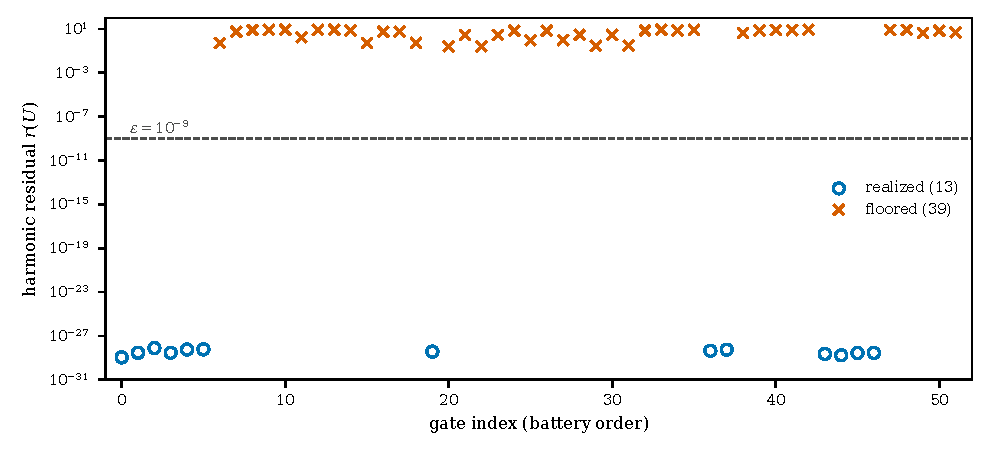
\includegraphics[width=\columnwidth]{fig-gate-battery}
\caption{The $52$-gate battery scored by the harmonic residual $r(U)$ of
the post-interaction state on the surgery-grown register. The $13$
charge-conserving gates reach machine zero ($r\sim10^{-29}$, blue
circles); the $39$ others floor at $r=0.2$--$8.5$ (orange crosses), each
certified by a nonzero period leak $|\Sigma|$. The dashed line is the
acceptance threshold $\epsilon=10^{-9}$.}
\label{fig:battery}
\end{figure}

Two control experiments delimit the result. In the Dijkgraaf--Witten
calibration layer (Sec.~\ref{sec:dw}), with the boundary pinned
bitwise-identically on a fixed twisted cylinder, the realizable image is
exactly $S_3$ --- the finite image expected of an abelian theory
\cite{Freedman2003TQC,NaiduRowell2011PropertyF}; synthesizing the boundary
is what lifts the integrality constraint and replaces the finite list with
the continuous group of Corollary~\ref{cor:gateset}. And the theorem is
implementation-robust across topologies: a randomized search over $3000$
surgery-grown bulks (subdivided spherical seeds, varied hole triples,
extra cuts), extended by $300$ further draws that also \emph{add} up to
$20$ vertices per draw by composed stellar subdivision, finds
$1282+161=1443$ genuine registers --- every one realizing exactly the
criterion set, as Corollary~\ref{cor:gateset} requires --- while the
remaining $1857$ draws fall outside Proposition~\ref{prop:register}'s
hypothesis and saturate the period space, dissolving the register rather
than carrying a new gate. The search thus confirms the theorem where its
hypothesis holds and charts the hypothesis boundary where it fails:
growing $b_1$, or refining the bulk, enlarges the realizable \emph{state}
space, never the \emph{gate} set.

\subsection{Transition amplitudes at machine precision}
\label{sec:results-h3}

Corollary~\ref{cor:h3} makes H3 an exact identity on the canonical bulk;
what remains to test is the implementation, and the test is sharp because
the identity admits no tolerance. The value reading of \eqref{eq:zspec}
was compared with the operator amplitude for every realized gate, on the
$V$-generic input and eight random carried states $\psi_A$ (nine pairs
per gate), with the Choi-channel amplitude computed independently as a
third reading (Table~\ref{tab:h3}).

\begin{table*}[t]
\centering
\small
\begin{tabular}{lrr}
\toprule
quantity & value & interpretation \\
\midrule
register Gram deviation $\max|G-I|$ & $7.8\times10^{-16}$ &
period map is a scaled isometry \\
worst $|\Zspec-\amp{\psi_A}{U}{\psi_B}|$ & $5.0\times10^{-16}$ &
H3, all 13 gates $\times$ 9 pairs \\
Choi-reading agreement & $1.6\times10^{-16}$ & independent operator route \\
equivariant re-triangulation drift & $9.7\times10^{-16}$ &
bulk independence (one subdivision) \\
generic-draw deviation vs.\ $a^\dagger(G-I)b$ & $\sim10^{-15}$ &
Gram defect predicts deviation \\
floored gates & no carried post-state & no value exists \\
\bottomrule
\end{tabular}
\caption{H3 at the value level, on the spectral data alone: the exact
identities of Sec.~\ref{sec:theorems} realized by the implementation.
One scale is fixed by the identity anchor on the reference input; every
subsequent number is a prediction. The re-triangulation row is exact on
the single symmetry-preserving subdivision tested; the generic-draw row
covers two anisotropic draws, whose deviation is the proven
law~\eqref{eq:deviation}.}
\label{tab:h3}
\end{table*}

\emph{The register chart is an isometry, as
Proposition~\ref{prop:isometry} requires.} The Gram matrix of the period
map $V\to\kerL_1$, in a flat-orthonormal basis of the $\Sigma=0$
hyperplane, is the identity to $7.8\times10^{-16}$. The hypothesis is
verified, not assumed: the canonical holes are a $C_3$ face-axis orbit
(Remark~\ref{rem:schur}), so the measured Gram is the implementation
check of a theorem --- any deviation beyond rounding would falsify the
eigendecomposition pipeline, not the proposition.

\emph{The value equals the amplitude.} Across all $13$ realized gates and
all pairs, the worst deviation between the anchored Hodge pairing and the
operator amplitude is $5.0\times10^{-16}$; the independent Choi-channel
reading agrees to $1.6\times10^{-16}$. Corollary~\ref{cor:h3}'s identity
is realized at machine precision, and transition probabilities
$|\Zspec|^2$ agree with $|\amp{\psi_A}{U}{\psi_B}|^2$ at the same order.
The identity row is the anchor's consistency check (the cylinder
reproduces the inner product on every carried pair), and the remaining
twelve gates are parameter-free predictions.

\emph{Bulk independence, with its mechanism.} The geodesic subdivision
with each holonomy hole re-placed on the central child of its original
face inherits the $C_3$ (Remark~\ref{rem:schur}), so
Proposition~\ref{prop:isometry} \emph{requires} the value to carry over
exactly --- and it does (Gram deviation $7.6\times10^{-16}$, value drift
$9.7\times10^{-16}$): the spectral form of triangulation invariance,
here a consequence of symmetry rather than an independent axiom. Two
generic hole draws still realize the same gates (Corollary~\ref
{cor:gateset} is symmetry-blind), but their period charts are anisotropic
(Gram defects $0.11$ and $0.25$), and their value deviations ($0.14$,
$0.26$) equal the exact law \eqref{eq:deviation} to $\sim10^{-15}$. The
value-level correspondence is thus the conservation law \emph{plus} the
isometric chart: surgery decides which gates are carried, symmetry makes
the carried pairing be the amplitude.

\emph{Obstruction at the value level.} A floored gate's post-interaction
state leaves the carried register; no harmonic representative exists, and
the operation has no value at all rather than a wrong one
(Corollary~\ref{cor:h3}) --- the value-level form of the residual-floor
certificate.

\subsection{Cross-calibration against a state-sum invariant}
\label{sec:dw}

The construction was historically calibrated against the $\mathbb{Z}_2$
Dijkgraaf--Witten state sum
\cite{DijkgraafWitten1990Topological,Wakui1992DWInvariant,FreedQuinn1993FiniteGauge}:
on torus-cylinder (identity) fixtures with longitude-aligned boundary
states --- the DW-representable subset, and only there --- the three
readings $\ZDW$, the operator amplitude, and $\Zspec$ agree to
$\sim10^{-15}$, while a generic $U(4)$ is uniformly bounded away from the
integer-quantized DW image (median gap $1.03$ over $200$ Haar samples).
The state-sum invariant is recovered as the quantized shadow of the
continuous spectral value --- they coincide exactly where the operation
lands on the flat-connection lattice --- and no state-sum machinery enters
the method itself.

\section{Discussion}
\label{sec:discussion}

\emph{What is established.} A variational, certificate-bearing decision
procedure for the existence of a discrete bulk realizing a given quantum
operation; a \emph{proven} characterization of the realizable gate set on
a $\mathbb{Z}_2$ holonomy register (Proposition~\ref{prop:register},
Lemma~\ref{lem:criterion}), with the implementation confirming the
theorem on every genuine register in thousands of randomized bulk draws
and both growth polarities; and a \emph{proven} value identity --- a
cyclic hole symmetry, verified for the canonical bulk, forces the
anchored harmonic pairing to \emph{be} the transition amplitude
(Proposition~\ref{prop:isometry}, Corollary~\ref{cor:h3}) --- validated
end-to-end at $5.0\times10^{-16}$, with bulk independence forced by the
lifted symmetry on the re-triangulation tested and the failure on
asymmetric bulks obeying the exact law~\eqref{eq:deviation}.

\emph{What is not claimed.} The register is abelian ($\mathbb{Z}_2$, a
two-dimensional carried space), and ``realized'' refers to a gate's
carried register action, not the full two-qubit unitary. The synthesized
bulks are simplicial complexes with pinned boundary, not verified PL
manifolds --- no link condition is checked, the H1 witnesses are weighted
graphs, and randomized surgery draws need not remain manifolds; the bulk
dimension varies by layer. The named count of realizable gates tracks the
chosen battery, not the physics. The symmetry hypothesis of
Proposition~\ref{prop:isometry} is sufficient, not necessary: which
asymmetric bulks also furnish isometric charts is charted only
empirically. The theorems cover the register layer; the oracle layer's
obstruction floors (Sec.~\ref{sec:results-h1}) remain numerical
certificates. The construction is a correspondence on finite complexes,
not a claim about continuum quantum gravity. Deciding whether $\kerL_k$
is nontrivial is QMA$_1$-hard for implicitly specified complexes
\cite{CrichignoKohler2024Clique}; the verdicts here are exact linear
algebra on small explicit complexes, and no efficiency claim is made ---
the multi-restart optimization with floor certificates is an architecture
matched to a problem that is hard in general, not a polynomial algorithm.

\emph{Outlook.} Two directions follow directly. First, a complete
obstruction theory for the oracle layer: the register layer now has one
(Sec.~\ref{sec:theorems}), and the resistor-network precedent
\cite{CurtisIngermanMorrow1998Circular} suggests the general
eigenvector-residual floors should likewise be replaced by provable
obstructions. Second, mediated synthesis: scoring candidate
bulks by a combined objective $F_\beta=r_U(W)+\beta S_{\mathrm{Regge}}(W^*)$
couples realizability to discrete gravitational action on the dual
complex, turning the present oracle into a laboratory for geometry
selection among the many bulks that realize a given operation; the
dimension lift of Remark~\ref{rem:dimension} supplies the substrate on
which the gravitational term has stationary points to select.

\section{Methods and reproducibility}
\label{sec:methods}

All experiments are pure orchestration of separately tested components of
the open-source \texttt{tessera} package:\footnote{The experiments are
\texttt{examples/cobordism/realizability\_report.py} and
\texttt{examples/cobordism/spectral\_gate\_realizability.py} (flags
\texttt{--h3} for the value validation; \texttt{--retries N --jobs 10}
for the randomized topology search, seeded with the script default
\texttt{--seed 12345}; \texttt{--max-additional-vertices}, default 20,
for the additive budget). The test suite (\texttt{pytest tests/cobordism})
pins the structural invariants and headline tolerances --- the criterion
set and its membership, the floor and leak certificates, the anchor
staging, and the H3 value invariants; the randomized-search tallies and
the figure-level digits come from the archived example runs.}
Choi--Jamio{\l}kowski bending; metric Hodge Laplacians at $k=0$ and
$k\ge1$; a fixed-boundary synthesis engine exposing interior weights,
stellar growth, interior-cell surgery with restore, and exact
eigendecomposition; and a bounded multi-restart Levenberg--Marquardt
fill. Conventions: operators are flat row-major; $k\ge1$ metric weights
are signed simplex volumes; acceptance $\epsilon=10^{-10}$ (oracle) and
$10^{-9}$ (register layer); obstruction floors are cross-checked against
an independent dense minimization; boundaries are pinned and verified
bitwise-identical through every move.

\section*{Code and data availability}
The implementation, experiment scripts, and test suite are available at
\url{https://github.com/akellehe/tessera}. Raw run tables for the
headline experiments (the gate battery with the H3 value validation, the
additive-search tally, and the realizability sweeps) are archived on the
repository's \texttt{issue-attachments} release; all tables regenerate
deterministically from the seeded example scripts.
% TODO before submission: tag a release at the exact commit the numbers
% were produced from (optionally mint a Zenodo DOI) and cite it here.

\section*{Acknowledgments}
The author received no specific funding for this work.
% TODO: confirm funding/acknowledgment text.

\bibliographystyle{quantum}
\bibliography{references}

\end{document}
